\section{Simple Output Geometry Is Not Sufficient}
\label{sec:geometry}

The family residual may still be a simple artifact of the top-1 decision rule.
KL and NLL summarize the full predictive distribution, whereas $D_S$ depends
on whether a perturbation crosses the local argmax boundary. We therefore test
a frozen sequence of non-tautological output-geometry models on the corrected
103-cell support set.

The baseline model conditions on the functional-damage summary and fixed
run/checkpoint/layer effects. Adding the intact top-1 margin alone does not
change the family coefficient. Adding anchored boundary displacement also
fails to shrink it: the estimated magnitude grows by 1.49\%. A full block that
adds logit-change norm and absolute alignment reduces the family coefficient by
20.18\%, from approximately $-0.0168$ to $-0.01344$ (95\% interval
$[-0.01764,-0.00923]$). The point estimate remains outside the frozen
equivalence region, although its interval overlaps the boundary slightly.

The partial shrinkage is accompanied by counterevidence to a simple boundary
story. An outcome-blind geometry-matched subset covers 31/103 cells and retains
a residual of $-0.02436$ (95\% interval $[-0.03006,-0.01819]$). The geometry
features do not pass the frozen sign-reversal prediction gate (leave-one-run-out
AUC 0.664), and layer heterogeneity increases by 26.2\% after adjustment rather
than decreasing. The far-margin stratum is near zero, but the effect is largest
at medium rather than nearest margins.

\begin{figure*}[t]
\centering
\begin{minipage}[t]{0.48\textwidth}\centering
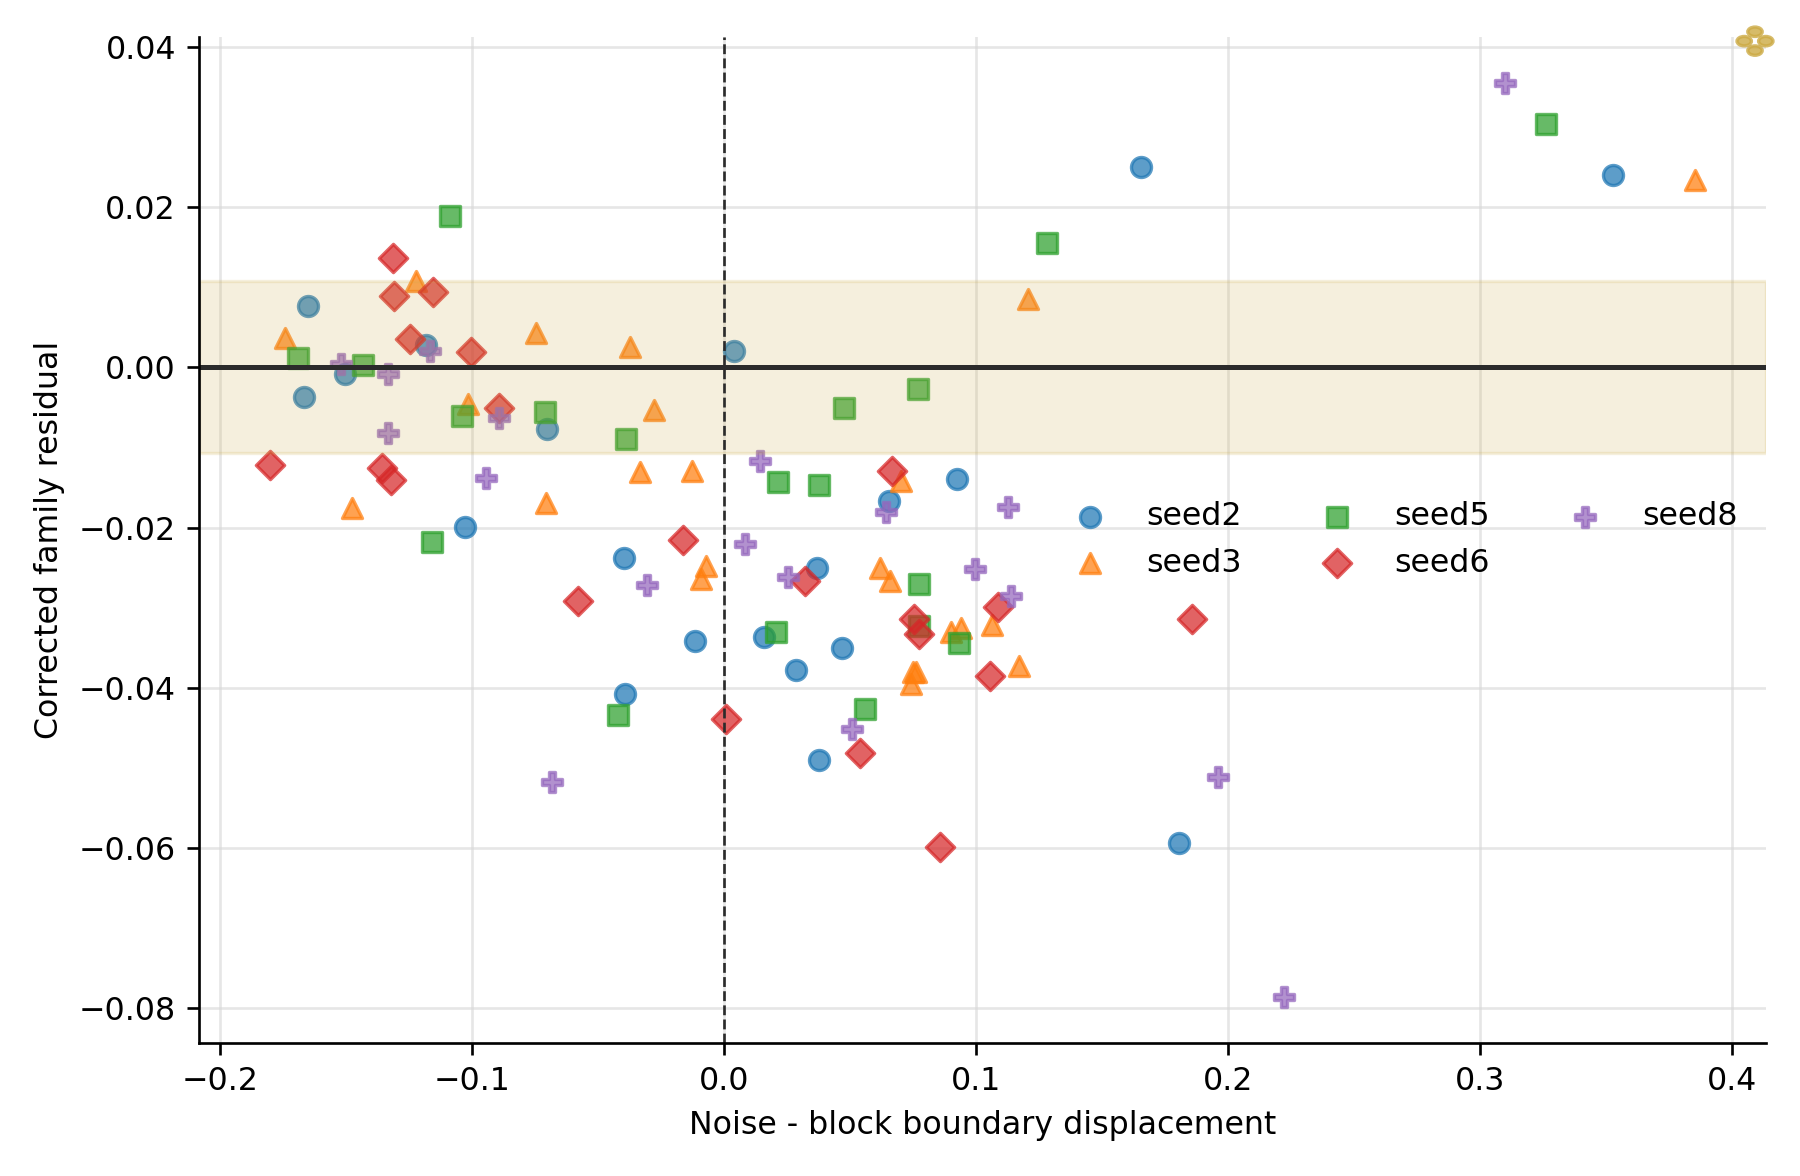
\includegraphics[width=\linewidth]{figures/draft2/fig4_residual_boundary.png}
\\[-2mm]\small (a) Frozen model sequence and residual shrinkage
\end{minipage}\hfill
\begin{minipage}[t]{0.48\textwidth}\centering
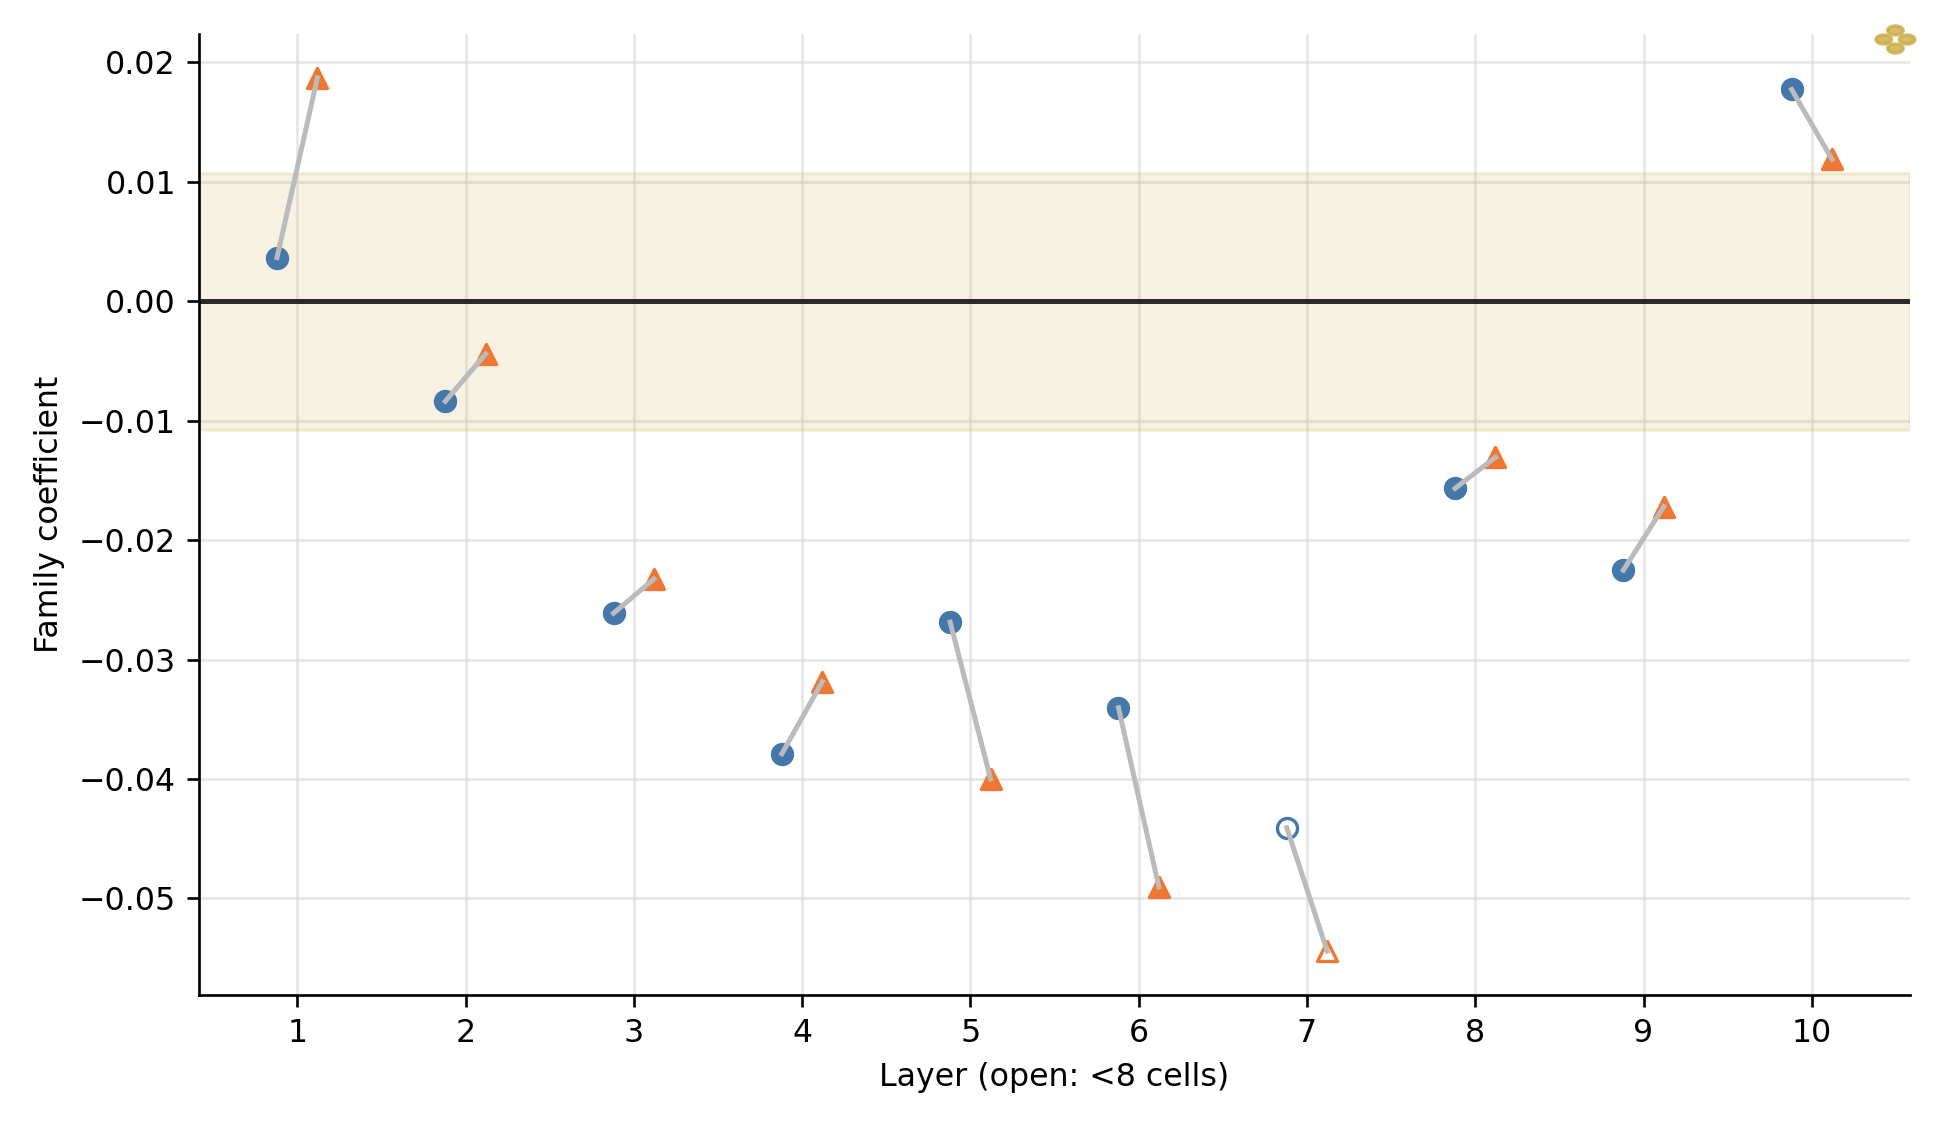
\includegraphics[width=\linewidth]{figures/draft2/fig4_layer_adjustment.png}
\\[-2mm]\small (b) Layer-level residual before and after geometry adjustment
\end{minipage}
\caption{\textbf{Output geometry is associated with only part of the family
residual.} The full frozen geometry block reduces the aggregate coefficient,
but the adjusted residual and heterogeneous layer structure remain. These are
associational controls, not a causal decomposition.}
\label{fig:geometry}
\end{figure*}

We conclude that the tested output geometry is incomplete. We do not conclude
that a deeper internal direction causes the remainder.
